\chapter{Kramers-Kronig Relations: COMING SOON}
\label{ch-kramers-kronig}

This chapter is mostly based on Ref.\cite{wiki-KKR}.  PP will stand for principal part. 

$\Re(z)=z_R$, $\Im(z)=z_I$ for any $z\in\CC$.

\beq
\chi(\omega)=
\int_{-\infty}^\infty dt\; e^{i\omega t}\chi(t)
\eeq

\beq
\chi(t)=
\int_{-\infty}^\infty \frac{d\omega}{2\pi}\; e^{-i\omega t}\chi(\omega)
\eeq

\beq
\delta(t) = \int_{-\infty}^\infty \frac{d\omega}{2\pi}e^{i\omega t}
\eeq

\beqa
\int_{-\infty}^\infty dt\; e^{i\omega t}
\int_{-\infty}^\infty \frac{d\omega'}{2\pi}\; e^{-i\omega' t}\chi(\omega')
&=&
\int_{-\infty}^\infty {d\omega'}
\underbrace{\left[
\int_{-\infty}^\infty \frac{dt}{2\pi}\;e^{i(\omega-\omega')t}
\right]}_{\delta(\omega-\omega')}
\chi(\omega')
\\
&=&
\chi(\omega)
\eeqa

\begin{figure}[h!]
$$
\begin{array}{ccc}
\xymatrix{
\chi(t_1)\ar[d]|{e^{i\omega_1 t_1}}
\ar[dr]\ar[drr]
&\chi(t_2)\ar[dl]\ar[d]\ar[dr]
&\chi(t_3)\ar[dll]\ar[dl]\ar[d]
\\
\chi(\omega_1)
&\chi(\omega_2)
&\chi(\omega_3)
}
&&
\xymatrix{
\chi(t_1)
&\chi(t_2)
&\chi(t_3)
\\
\chi(\omega_1)\ar[u]|{e^{-i\omega_1 t_1}}
\ar[ur]
\ar[urr]
&\chi(\omega_2)\ar[ul]\ar[u]\ar[ur]
&\chi(\omega_3)\ar[ull]\ar[ul]\ar[u]
}
\\
\\
(a) && (b)
\end{array}
$$
\caption{$(a)$ bnet for Fourier Transform, $(b)$ bnet
for Inverse Fourier Transform}
\label{fig-fourier-bnet}
\end{figure}



\begin{claim}
$\chi(t)=0$ for $t<0$ $\iff$ $\chi(\omega)$ is analytic 
in upper half of the $\omega$ complex plane
and tends to zero there as $|\omega|\rarrow \infty$.
\end{claim}
\proof

Motivation (not rigorous proof)

\beq
\chi(\omega)=
\int_{0}^\infty dt\; e^{i\omega t}\chi(t)
\eeq
Assume $t>0$.
When $\omega=i\omega_I$, with $\omega_I>0$ 
(upper half complex $\omega$ plane), $i\omega t= -\omega_I t<0$.
Thus $e^{i\omega t}\rarrow 0$ as $t\rarrow \infty$.
This means it has no singularities at infinity. It's also smooth
(i.e., no singularities like poles or essential singularities)
for $\omega$ in upper half plane for finite $|\omega|$.
\qed

\begin{claim}
$\chi(t)$ is real $\iff$ $\chi^*(-\omega)=\chi(\omega)$

$\iff$
$\left\{
\begin{array}{ll} 
\chi_R(-\omega) =\chi_R(\omega)
&\text{(even function)}
\\
\chi_I(-\omega) =-\chi_I(\omega)
&\text{(odd function)}
\end{array} 
\right\}$
\end{claim}
\proof

\beq
\chi(\omega)=
\int_{-\infty}^\infty dt\; e^{i\omega t}\chi(t)
\eeq
When $\chi(t)$ is real,

\beq
\chi^*(-\omega)= 
\int_{-\infty}^\infty dt\; e^{-i(-\omega) t}\chi(t)=\chi(\omega)
\eeq

\qed

\begin{claim}(Kramers-Kronig relations)

If $\chi(\omega)$ is analytic 
in the upper half of the $\omega$ complex plane
and tends to zero there as $|\omega|\rarrow \infty$, then:

\beq
\chi(\omega) = \frac{1}{i\pi}
{\rm PP} \int_{-\infty}^\infty d\omega'\;
\frac{\chi(\omega')}{\omega'-\omega}
\eeq
The latter immediately implies:

\beq
\chi_R(\omega) = \frac{1}{\pi}{\rm PP}
\int_{-\infty}^{\infty}d\omega'\; 
\frac{\chi_I(\omega')}{\omega'-\omega}
\label{eq-R-equals-int-I}
\eeq

\beq
\chi_I(\omega) = -\frac{1}{\pi}{\rm PP}
\int_{-\infty}^{\infty}d\omega'\; 
\frac{\chi_R(\omega')}{\omega'-\omega}
\label{eq-I-equals-int-R}
\eeq

\end{claim}
\proof

\begin{figure}[h!]
\centering
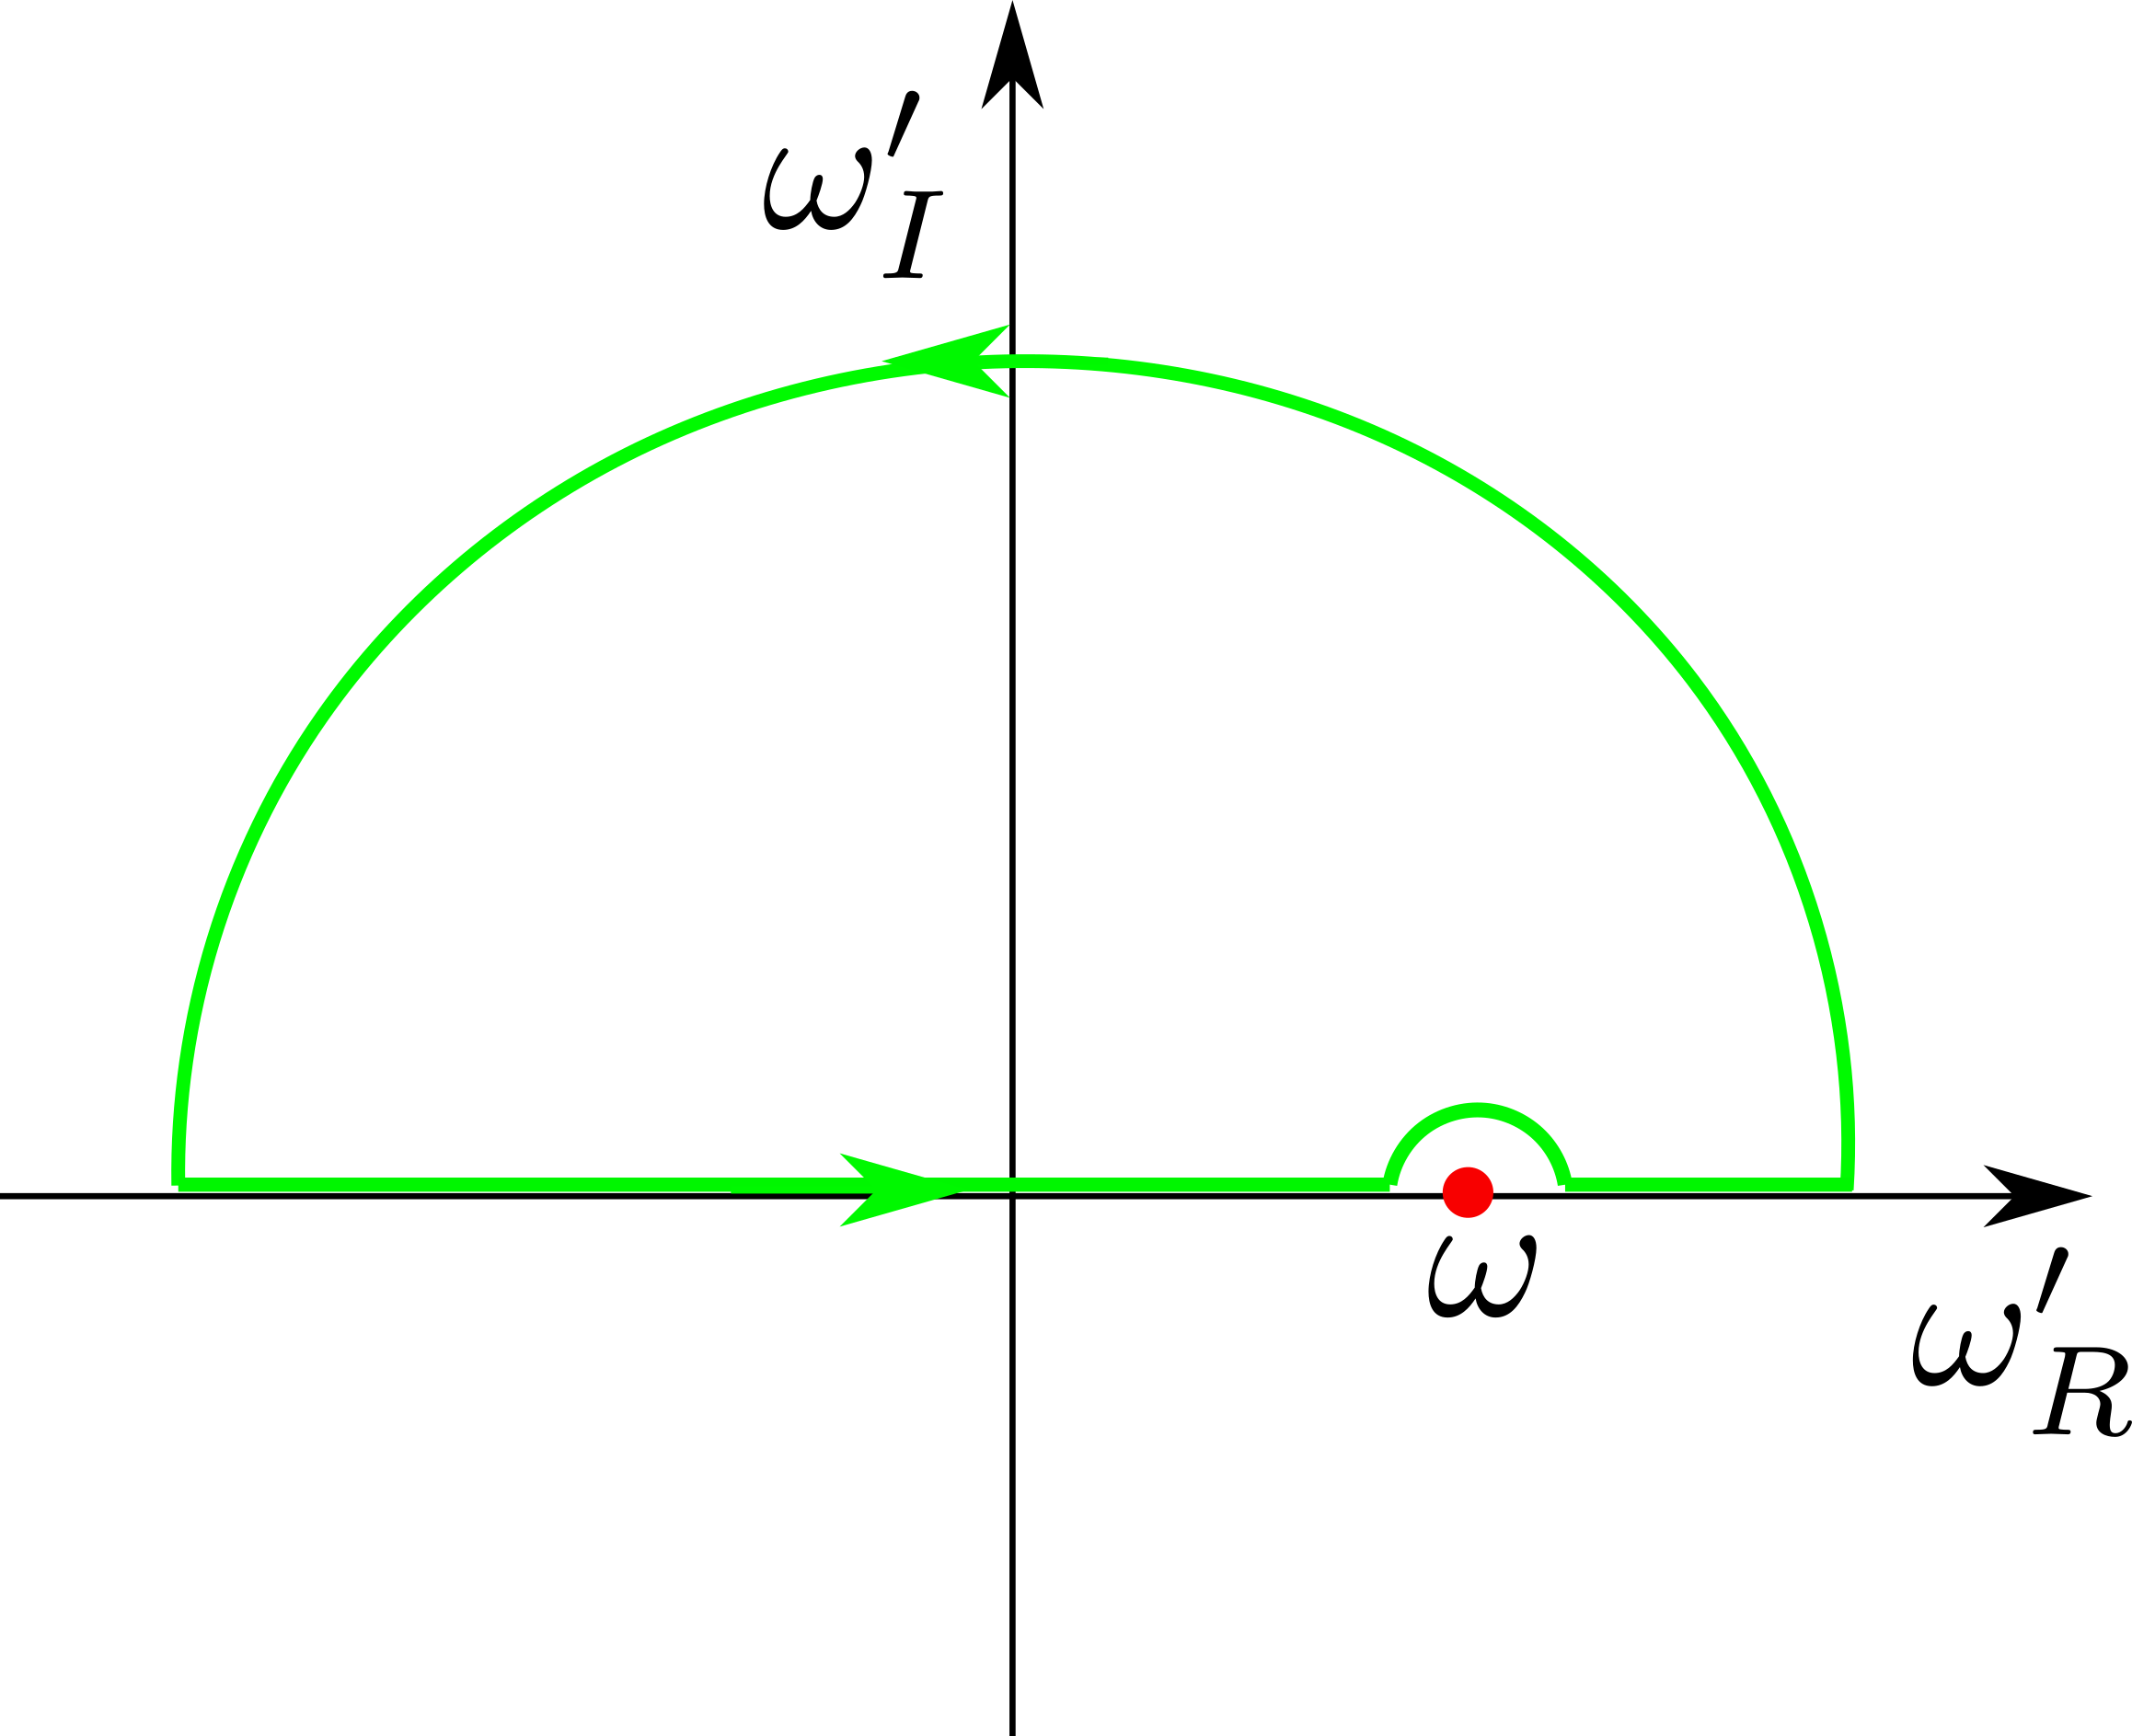
\includegraphics[width=2in]
{kramers-kronig/closed-path.png}
\caption{Integration contour in $\omega'$ complex
plane. Used to prove Kramers-Kronig relations.}
\label{fig-closed-path-kkr}
\end{figure}

\beq
\int_{\gamma}d\omega'
 \frac{\chi(\omega')}{\omega'-\omega} =0
\eeq

\beq
\omega'-\omega = \rho e^{i\theta}
\eeq

\beqa
\int_{SC}\frac{\chi(\omega')}{\omega'-\omega}
&=&
\chi(\omega)\int_{SC}\frac{d(\rho e^{i\theta})}{\rho e^{i\theta}}
\\
&=&
\chi(\omega)\int_{\pi}^{0}id\theta 
\\
&=&
\chi(\omega)(-i\pi)
\eeqa
 
\beq
0=\int_{\gamma}d\omega'
 \frac{\chi(\omega')}{\omega'-\omega} =
 PP
 \int_{\-\infty}^{\infty}d\omega'
  \frac{\chi(\omega')}{\omega'-\omega}
 -i\pi \chi(\omega)
\eeq

\qed

\begin{claim}(Kramers-Kronig relations assuming $\chi(t)$ is real)

If $\chi(t)$ is real, then need only integrate
over positive frequencies.

\beq
\chi_R =\frac{2}{\pi}
\int_0^\infty d\omega'\;\frac{\omega' \chi_I(\omega')}
{\omega^{'2}-\omega^2}
\eeq

\beq
\chi_I =-\frac{2}{\pi}
\int_0^\infty d\omega'\;\frac{\omega \chi_R(\omega')}
{\omega^{'2}-\omega^2}
\eeq
\end{claim}
\proof

Multiply by $(\omega'+\omega)$
the numerator and denominator
of the integrand of Eq.(\ref{eq-R-equals-int-I})
to get

\beqa
\chi_R(\omega) 
&=& \frac{1}{\pi}{\rm PP}
\int_{-\infty}^{\infty}d\omega'\; 
\frac{\chi_I(\omega')}{\omega'-\omega}
\\
&=&
 \frac{1}{\pi}{\rm PP}
\int_{-\infty}^{\infty}d\omega'\; 
\frac{(\omega'+\omega)\overbrace{\chi_I(\omega')}^{\text{odd function}}}{\omega^{'2}-\omega^2}
\\
&=&
 \frac{2}{\pi}{\rm PP}
\int_{0}^{\infty}d\omega'\; 
\frac{\omega'\chi_I(\omega')}{\omega^{'2}-\omega^2}
\eeqa

Multiply by $(\omega'+\omega)$
the numerator and denominator
of the integrand of Eq.(\ref{eq-I-equals-int-R})
to get

\beqa
\chi_I(\omega) 
&=& -\frac{1}{\pi}{\rm PP}
\int_{-\infty}^{\infty}d\omega'\; 
\frac{\chi_R(\omega')}{\omega'-\omega}
\\
&=&
 -\frac{1}{\pi}{\rm PP}
\int_{-\infty}^{\infty}d\omega'\; 
\frac{(\omega'+\omega)\overbrace{\chi_R(\omega')}^{\text{even function}}}{\omega^{'2}-\omega^2}
\\
&=&
- \frac{2}{\pi}{\rm PP}
\int_{0}^{\infty}d\omega'\; 
\frac{\omega\chi_R(\omega')}{\omega^{'2}-\omega^2}
\eeqa
\qed

\section{Damped Harmonic Oscillator Example}

From Chapter \ref{ch-greens-fun}

\beq
\call= \partial_t^2 x + 2\gamma \partial_t + \omega^2_0
\eeq

\beq
\call x = f(t)
\eeq

If 

\beq
x(t) = \int dt \chi(t, s)f(s)
\eeq


\beq
x(t) =\int_{-\infty}^{\infty}\frac{d\omega}{2\pi}
e^{-i\omega t}x(\omega)
\;,\quad
\delta(t) =
\int_{-\infty}^{\infty}\frac{d\omega}{2\pi}
e^{-i\omega t}
\eeq

\beq
x(\omega)(-\omega^{2} -i2\gamma\omega  +\omega_0^2)= 1
\eeq

\beq
\chi(\omega)=
\frac{1}{\omega_0^2-\omega^2 - i 2\gamma \omega}
\eeq

